% Options for packages loaded elsewhere
\PassOptionsToPackage{unicode}{hyperref}
\PassOptionsToPackage{hyphens}{url}
\PassOptionsToPackage{dvipsnames,svgnames,x11names}{xcolor}
%
\documentclass[
  letterpaper,
  DIV=11,
  numbers=noendperiod]{scrartcl}

\usepackage{amsmath,amssymb}
\usepackage{iftex}
\ifPDFTeX
  \usepackage[T1]{fontenc}
  \usepackage[utf8]{inputenc}
  \usepackage{textcomp} % provide euro and other symbols
\else % if luatex or xetex
  \usepackage{unicode-math}
  \defaultfontfeatures{Scale=MatchLowercase}
  \defaultfontfeatures[\rmfamily]{Ligatures=TeX,Scale=1}
\fi
\usepackage{lmodern}
\ifPDFTeX\else  
    % xetex/luatex font selection
\fi
% Use upquote if available, for straight quotes in verbatim environments
\IfFileExists{upquote.sty}{\usepackage{upquote}}{}
\IfFileExists{microtype.sty}{% use microtype if available
  \usepackage[]{microtype}
  \UseMicrotypeSet[protrusion]{basicmath} % disable protrusion for tt fonts
}{}
\makeatletter
\@ifundefined{KOMAClassName}{% if non-KOMA class
  \IfFileExists{parskip.sty}{%
    \usepackage{parskip}
  }{% else
    \setlength{\parindent}{0pt}
    \setlength{\parskip}{6pt plus 2pt minus 1pt}}
}{% if KOMA class
  \KOMAoptions{parskip=half}}
\makeatother
\usepackage{xcolor}
\setlength{\emergencystretch}{3em} % prevent overfull lines
\setcounter{secnumdepth}{-\maxdimen} % remove section numbering
% Make \paragraph and \subparagraph free-standing
\ifx\paragraph\undefined\else
  \let\oldparagraph\paragraph
  \renewcommand{\paragraph}[1]{\oldparagraph{#1}\mbox{}}
\fi
\ifx\subparagraph\undefined\else
  \let\oldsubparagraph\subparagraph
  \renewcommand{\subparagraph}[1]{\oldsubparagraph{#1}\mbox{}}
\fi


\providecommand{\tightlist}{%
  \setlength{\itemsep}{0pt}\setlength{\parskip}{0pt}}\usepackage{longtable,booktabs,array}
\usepackage{calc} % for calculating minipage widths
% Correct order of tables after \paragraph or \subparagraph
\usepackage{etoolbox}
\makeatletter
\patchcmd\longtable{\par}{\if@noskipsec\mbox{}\fi\par}{}{}
\makeatother
% Allow footnotes in longtable head/foot
\IfFileExists{footnotehyper.sty}{\usepackage{footnotehyper}}{\usepackage{footnote}}
\makesavenoteenv{longtable}
\usepackage{graphicx}
\makeatletter
\def\maxwidth{\ifdim\Gin@nat@width>\linewidth\linewidth\else\Gin@nat@width\fi}
\def\maxheight{\ifdim\Gin@nat@height>\textheight\textheight\else\Gin@nat@height\fi}
\makeatother
% Scale images if necessary, so that they will not overflow the page
% margins by default, and it is still possible to overwrite the defaults
% using explicit options in \includegraphics[width, height, ...]{}
\setkeys{Gin}{width=\maxwidth,height=\maxheight,keepaspectratio}
% Set default figure placement to htbp
\makeatletter
\def\fps@figure{htbp}
\makeatother

\KOMAoption{captions}{tableheading}
\makeatletter
\makeatother
\makeatletter
\makeatother
\makeatletter
\@ifpackageloaded{caption}{}{\usepackage{caption}}
\AtBeginDocument{%
\ifdefined\contentsname
  \renewcommand*\contentsname{Table of contents}
\else
  \newcommand\contentsname{Table of contents}
\fi
\ifdefined\listfigurename
  \renewcommand*\listfigurename{List of Figures}
\else
  \newcommand\listfigurename{List of Figures}
\fi
\ifdefined\listtablename
  \renewcommand*\listtablename{List of Tables}
\else
  \newcommand\listtablename{List of Tables}
\fi
\ifdefined\figurename
  \renewcommand*\figurename{Figure}
\else
  \newcommand\figurename{Figure}
\fi
\ifdefined\tablename
  \renewcommand*\tablename{Table}
\else
  \newcommand\tablename{Table}
\fi
}
\@ifpackageloaded{float}{}{\usepackage{float}}
\floatstyle{ruled}
\@ifundefined{c@chapter}{\newfloat{codelisting}{h}{lop}}{\newfloat{codelisting}{h}{lop}[chapter]}
\floatname{codelisting}{Listing}
\newcommand*\listoflistings{\listof{codelisting}{List of Listings}}
\makeatother
\makeatletter
\@ifpackageloaded{caption}{}{\usepackage{caption}}
\@ifpackageloaded{subcaption}{}{\usepackage{subcaption}}
\makeatother
\makeatletter
\@ifpackageloaded{tcolorbox}{}{\usepackage[skins,breakable]{tcolorbox}}
\makeatother
\makeatletter
\@ifundefined{shadecolor}{\definecolor{shadecolor}{rgb}{.97, .97, .97}}
\makeatother
\makeatletter
\makeatother
\makeatletter
\makeatother
\ifLuaTeX
  \usepackage{selnolig}  % disable illegal ligatures
\fi
\IfFileExists{bookmark.sty}{\usepackage{bookmark}}{\usepackage{hyperref}}
\IfFileExists{xurl.sty}{\usepackage{xurl}}{} % add URL line breaks if available
\urlstyle{same} % disable monospaced font for URLs
\hypersetup{
  pdftitle={About},
  colorlinks=true,
  linkcolor={blue},
  filecolor={Maroon},
  citecolor={Blue},
  urlcolor={Blue},
  pdfcreator={LaTeX via pandoc}}

\title{About}
\author{}
\date{}

\begin{document}
\maketitle
\ifdefined\Shaded\renewenvironment{Shaded}{\begin{tcolorbox}[frame hidden, boxrule=0pt, enhanced, interior hidden, borderline west={3pt}{0pt}{shadecolor}, breakable, sharp corners]}{\end{tcolorbox}}\fi

\texttt{Arkansas\ State\ University\ (ASU)\ is\ a\ public\ research\ university\ located\ in\ Jonesboro,\ Arkansas,\ United\ States.\ It\ is\ the\ flagship\ campus\ of\ the\ Arkansas\ State\ University\ System\ and\ offers\ a\ wide\ range\ of\ academic\ programs.}

Key details about Arkansas State University:

\begin{enumerate}
\def\labelenumi{\arabic{enumi}.}
\item
  \textbf{History:} ASU was established in 1909 as the First District
  Agricultural School. Over the years, it evolved into a four-year
  college and later became a university. It adopted its current name,
  Arkansas State University, in 1967.
\item
  \textbf{Campus:} The main campus of ASU is situated on 1,376 acres in
  Jonesboro, a city in northeastern Arkansas. The campus features modern
  academic buildings, residence halls, recreational facilities, and
  green spaces.
\item
  \textbf{Academic Programs:} ASU offers a comprehensive range of
  undergraduate and graduate programs across various disciplines. It has
  colleges and schools dedicated to fields such as Agriculture,
  Business, Education and Behavioral Science, Engineering and Computer
  Science, Liberal Arts and Communication, Nursing and Health
  Professions, Sciences and Mathematics, and Honors College.
\item
  \textbf{Research and Innovation:} ASU is a research-intensive
  institution with a strong focus on applied research and innovation. It
  promotes collaborative research projects and encourages students to
  engage in hands-on research experiences.
\item
  \textbf{Athletics:} ASU's athletic teams, known as the Arkansas State
  Red Wolves, compete in the NCAA Division I Sun Belt Conference. The
  university has a strong athletic program and fields teams in sports
  such as football, basketball, baseball, soccer, track and field, and
  more.
\item
  \textbf{Student Life:} ASU has a vibrant campus life with numerous
  student organizations, clubs, and activities. There are opportunities
  for involvement in areas like leadership development, community
  service, cultural events, and recreational pursuits.
\item
  \textbf{Facilities:} The university boasts modern facilities,
  including state-of-the-art classrooms, laboratories, libraries, and
  athletic complexes. ASU also has an on-campus museum, the Arkansas
  State University Museum, which showcases exhibits on regional history
  and art.
\item
  \textbf{Community Engagement:} ASU actively engages with the local
  community through various outreach initiatives. It collaborates with
  businesses, government agencies, and nonprofit organizations to
  address regional needs and contribute to the economic and social
  development of the area.
\end{enumerate}

\texttt{ASU\ has\ a\ reputation\ for\ academic\ excellence,\ commitment\ to\ research,\ and\ fostering\ student\ success.\ It\ serves\ as\ an\ educational\ and\ cultural\ hub\ in\ northeastern\ Arkansas,\ offering\ a\ diverse\ and\ inclusive\ learning\ environment.}

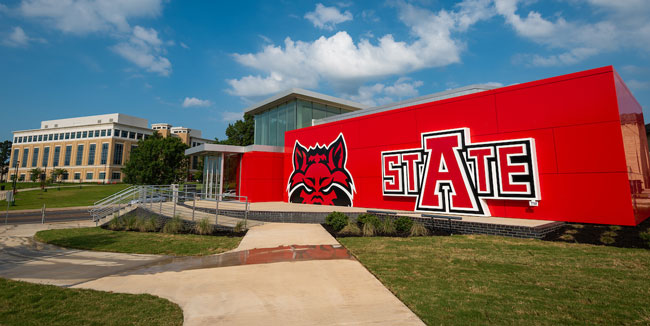
\includegraphics{Welcome-Center-web.jpeg}



\end{document}
